\documentclass{beamer}

\mode<presentation> {

%\usetheme{default}
%\usetheme{AnnArbor}
%\usetheme{Antibes}
%\usetheme{Bergen}
%\usetheme{Berkeley}
%\usetheme{Berlin}
%\usetheme{Boadilla}
%\usetheme{CambridgeUS}
%\usetheme{Copenhagen}
%\usetheme{Darmstadt}
%\usetheme{Dresden}
%\usetheme{Frankfurt}
%\usetheme{Goettingen}
%\usetheme{Hannover}
%\usetheme{Ilmenau}
%\usetheme{JuanLesPins}
%\usetheme{Luebeck}
\usetheme{Madrid}
%\usetheme{Malmoe}
%\usetheme{Marburg}
%\usetheme{Montpellier}
%\usetheme{PaloAlto}
%\usetheme{Pittsburgh}
%\usetheme{Rochester}
%\usetheme{Singapore}
%\usetheme{Szeged}
%\usetheme{Warsaw}


%\usecolortheme{albatross}
%\usecolortheme{beaver}
%\usecolortheme{beetle}
%\usecolortheme{crane}
%\usecolortheme{dolphin}
%\usecolortheme{dove}
%\usecolortheme{fly}
%\usecolortheme{lily}
%\usecolortheme{orchid}
%\usecolortheme{rose}
%\usecolortheme{seagull}
%\usecolortheme{seahorse}
%\usecolortheme{whale}
%\usecolortheme{wolverine}

%\setbeamertemplate{footline} % To remove the footer line in all slides uncomment this line
%\setbeamertemplate{footline}[page number] % To replace the footer line in all slides with a simple slide count uncomment this line

%\setbeamertemplate{navigation symbols}{} % To remove the navigation symbols from the bottom of all slides uncomment this line
}

\usepackage{graphicx} % Allows including images
\usepackage{booktabs} % Allows the use of \toprule, \midrule and \bottomrule in tables
\usepackage{amsfonts}
\usepackage{mathrsfs, bbold}
\usepackage{amsmath,amssymb,graphicx}
\usepackage{mathtools} % gather

%----------------------------------------------------------------------------------------
%	TITLE PAGE
%----------------------------------------------------------------------------------------

\title["6"]{6: Model Checking}

\author{Taylor} 
\institute[UVA] 
{
University of Virginia \\
\medskip
\textit{} 
}
\date{} 

\begin{document}
%----------------------------------------------------------------------------------------

\begin{frame}
\titlepage 
\end{frame}

%----------------------------------------------------------------------------------------
\begin{frame}
\frametitle{Introduction}

Now we finally admit some of the uncertainty we have about our choices of likelihood and prior distribution. Instead of asking ``is our  model true," we ask ``are our inferences being substantially affected by the model's deficiencies?"
\newline

We are either making inferences on unobservable $\theta$ with $p(\theta \mid y)$, or *potentially* observable data with $p(\tilde{y} \mid y)$. This means it's generally easier to check inferences on the latter!

\end{frame}

%----------------------------------------------------------------------------------------
\begin{frame}
\frametitle{Notation Clarification}

There is now a difference between $y^{\text{rep}}$ and $\tilde{y}$!
\newline

\begin{enumerate}
\item $y$: the data we have observed and have made inferences using
\item $y^{\text{rep}}$: data simulated from the posterior predictive distribution (ppd)
\item $\tilde{y}$: actual future data, possibly coming from the \*true\* model we aren't using
\item $p(y^{\text{rep}} \mid y)$ our ``working" ppd that we are examining and are unsure about
\end{enumerate}


\end{frame}


%----------------------------------------------------------------------------------------
\begin{frame}
\frametitle{External Validation}

The gold standard for evaluating the posterior predictive distribution is {\bf external validation}, which is when you compare actual future data $\tilde{y}$ with your predictions coming from $p(y^{\text{rep}} \mid y)$.
\newline

In general, we might want to predict $T(\tilde{y})$, where $T$ is some arbitrary test function of a new data (set) $\tilde{y}$.
\newline

In a time series context: predict, wait for new data to arrive, compare.
\newline

In a non-time series context: predict, wait for new data to be collected, compare.

\end{frame}

%----------------------------------------------------------------------------------------
\begin{frame}
\frametitle{Posterior Predictive Checks}

When we can't/won't wait for new data to arrive, we can use our existing data set $y$ by calculating a {\bf posterior predictive p-value} $p_B$. 
\newline

\[
p_B = P(T(y^{\text{rep}}) > T(y) \mid y) = \int_{\{T(y^{\text{rep}}) : T(y^{\text{rep}}) > T(y) \}} p(y^{\text{rep}} \mid y) \text{d}y^{\text{rep}}. 
\]

\begin{enumerate}
\item if $p_b = .5$, the median of $p(T(y^{\text{rep}}) \mid y)$ is exactly equal to $T(y)$.
\item if $p_b > .5$, the median of $p(T(y^{\text{rep}}) \mid y)$ is greater than  $T(y)$.
\item if $p_b < .5$, the median of $p(T(y^{\text{rep}}) \mid y)$ is less than  $T(y)$
\end{enumerate}



\end{frame}




%----------------------------------------------------------------------------------------
\begin{frame}
\frametitle{Posterior Predictive Checks}

$p_b = .5$ does not \*prove\* your model is good! 
\begin{enumerate}
\item Maybe you're overfitting. Remember, you're using the data twice.
\item Maybe you're using an "easy" test function (e.g. a sufficient statistic).
\item Maybe it does poorly for other test functions.
\end{enumerate}

\end{frame}


%----------------------------------------------------------------------------------------
\begin{frame}
\frametitle{Posterior Predictive Checks}

We can extend this a bit further:

\[
p_B = P(T(y^{\text{rep}}, \theta) > T(y, \theta) \mid y) = \iint_{A} p(y^{\text{rep}}, \theta \mid y) \text{d} y^{\text{rep}}\text{d} \theta
\]

where $A = \{T(y^{\text{rep}}, \theta) : T(y^{\text{rep}}, \theta) > T(y, \theta) \}$

\end{frame}



%----------------------------------------------------------------------------------------
\begin{frame}
\frametitle{Posterior Predictive Checks}

When we can't/won't evaluate this integral, we can use Monte Carlo!

\begin{align*}
p_B &= \iint_{A} p(y^{\text{rep}}, \theta \mid y) \text{d} y^{\text{rep}}\text{d} \theta \\
&= E \left[ \mathbf{1}( (y^{\text{rep}}, \theta) \in A) \mid y\right] \\
&\leftarrow S^{-1}\sum_{i=1}^S \mathbf{1}( (y^{i,\text{rep}}, \theta^i) \in A) 
\end{align*}
where 

If we can't simulate directly from the ppd, then we can do the following. \\
For $i=1,\ldots,S$
\begin{enumerate}
\item Simulate $\theta^i \sim p(\theta \mid y)$
\item Simulate $y^{i,\text{rep}} \sim p(y \mid \theta^i)$
\item Count up the number of times $(y^{i,\text{rep}}, \theta^i) \in A$
\item Divide that number by $S$
\end{enumerate}

\end{frame}

%----------------------------------------------------------------------------------------
\begin{frame}
\frametitle{Notation}

NB: I try to use superscripts for draws, and subscripts for indexes in a particular data set.
\newline

Example: $y^{i,\text{rep}}$ is the $i$th replicated data set
\newline

Example: $y_i$ is the $i$th element of one data set

\end{frame}

%----------------------------------------------------------------------------------------
\begin{frame}
\frametitle{Example: Speed of Light Measurements}

A histogram of $y$
\begin{center}
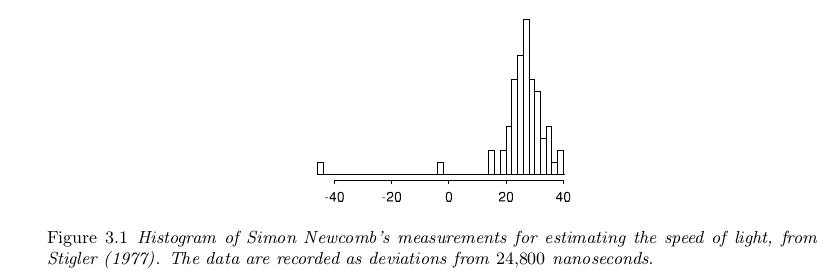
\includegraphics[width=120mm]{speed_light_data.png}
\end{center}

\end{frame}


%----------------------------------------------------------------------------------------
\begin{frame}
\frametitle{Example: Speed of Light Measurements}

\begin{enumerate}
\item $y$: $66$ univariate measurements 
\item $p(y \mid \mu, \sigma^2) = \prod_{i=1}^{66}\text{Normal}(y_i \mid \mu, \sigma^2)$
\item $p(\mu, \sigma^2) \propto \sigma^{-2}$
\item $j = 1, \ldots, 20$ simulations
\item each $y^{i, \text{rep}}$ is a data set of size $66$ simulated from the ppd
\end{enumerate}


\end{frame}




%----------------------------------------------------------------------------------------
\begin{frame}[fragile]
\frametitle{Example: Speed of Light Measurements}

Let's simulate a data set $y^{\text{rep}} \sim p(y^{\text{rep}} \mid y)$
\newline

Recall from chapter 3:
\[
y^{\text{rep}} \mid y \sim t_{n-1}(\bar{y}, s^2(1 + 1/n)).
\]

\begin{verbatim}
n <- length(y)
s <- sd(y)
my <- mean(y)
sampt20 <- replicate(20, rt(n, n-1)*sqrt(1+1/n)*s+my) %>%
  as.data.frame()
dim(sampt20)
[1]   66 20
\end{verbatim}
\url{http://avehtari.github.io/BDA_R_demos/demos_ch6/demo6_1.html}
\end{frame}

%----------------------------------------------------------------------------------------
\begin{frame}
\frametitle{Example: Speed of Light Measurements}

Each one of these simulated data sets produces one univariate $T(y^{\text{rep}})$
\begin{center}
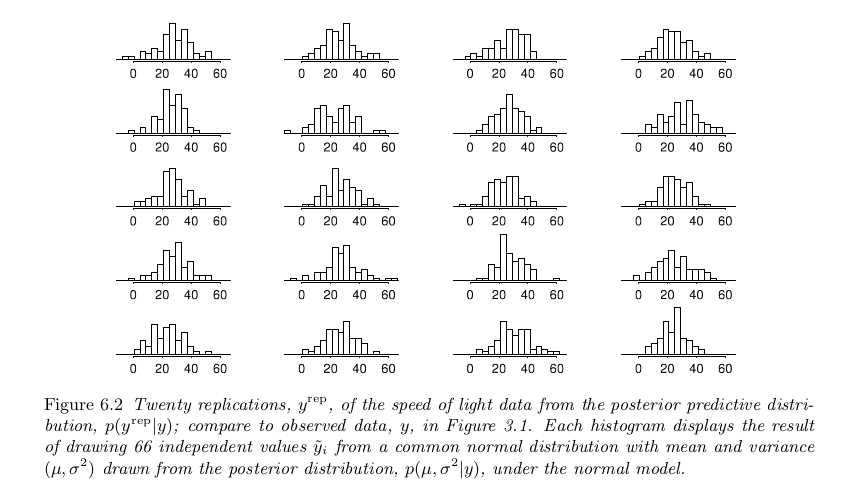
\includegraphics[width=120mm]{sim_data_sets.png}
\end{center}

\end{frame}


%----------------------------------------------------------------------------------------
\begin{frame}[fragile]
\frametitle{Example: Speed of Light Measurements}

Let $T(y^{j,\text{rep}}) = \min(y_1^{j,\text{rep}}, \ldots, y_n^{j,\text{rep}})$ and $T(y) = \min(y_1, \ldots, y_n)$. Then
\[
P(T(y^{\text{rep}}) > T(y) \mid y)  \approx 1000^{-1} \sum_{j=1}^{1000} \mathbf{1}\left(T(y^{j,\text{rep}}) > T(y) \right)
\]

\begin{verbatim}
sampt1000 <- replicate(1000, rt(n, n-1)*sqrt(1+1/n)*s+my) %>%
  as.data.frame()
mean(sapply(sampt1000, min) > min(y))
[1] 1
\end{verbatim}

\end{frame}


%----------------------------------------------------------------------------------------
\begin{frame}
\frametitle{Example: Speed of Light Measurements}

\begin{center}
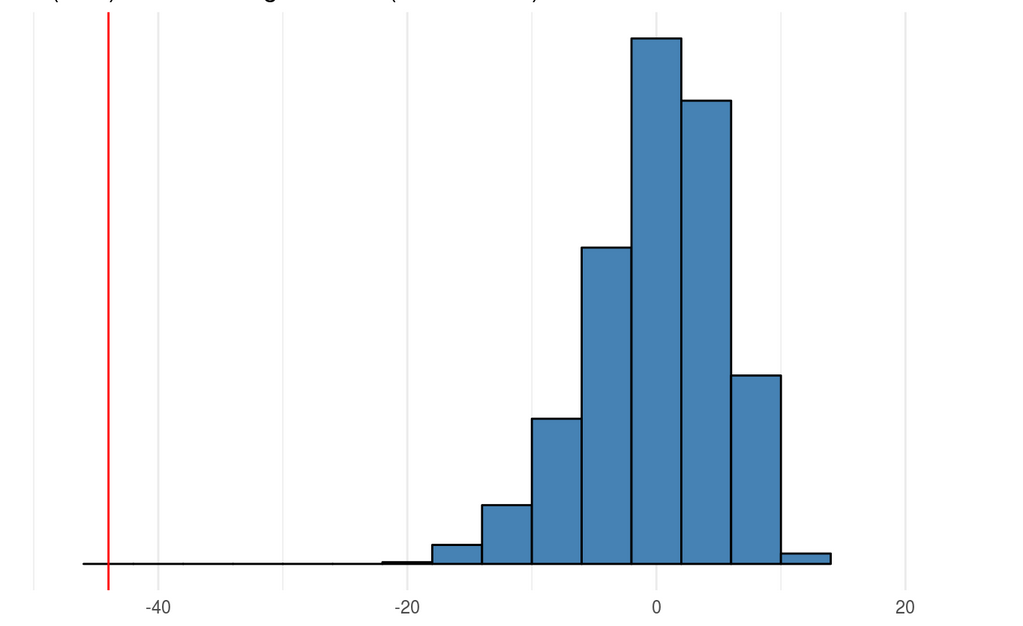
\includegraphics[width=120mm]{mins_histogram.png}
\end{center}

\end{frame}


%----------------------------------------------------------------------------------------
\begin{frame}
\frametitle{Example: Speed of Light Measurements}

Let $T(y) = |y_{(61)} - \theta| - |y_{(6)} - \theta|$

\begin{center}
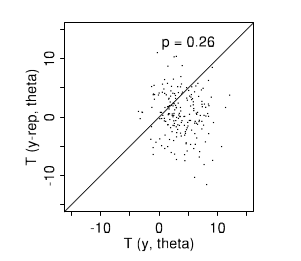
\includegraphics[width=80mm]{T_scatter.png}
\end{center}

\end{frame}

%----------------------------------------------------------------------------------------
\begin{frame}
\frametitle{Example: Speed of Light Measurements}

Let $T(y) = (n-1)^{-1}\sum_{i=1}^n (y_i-\bar{y})^2$

\begin{center}
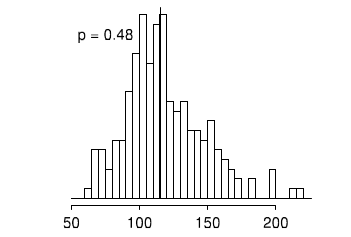
\includegraphics[width=80mm]{s2_hist.png}
\end{center}

Bayesian sufficiency implies ``predictive sufficiency" \\
$P(T(y^{\text{rep} } ) > T(y ) \mid y) = P(T(y^{\text{rep} } ) > T(y) \mid \bar{y}, T(y))$

%https://stats.stackexchange.com/questions/339075/how-does-bayesian-sufficiency-relate-to-frequentist-sufficiency/339076#339076

\end{frame}

%----------------------------------------------------------------------------------------
\begin{frame}
\frametitle{Example 2: Are our Bernoulli rvs Correlated?}

From chapter 2:
\begin{enumerate}
\item $y_1, \ldots, y_n \mid \theta \overset{\text{iid}}{\sim} \text{Bernoulli}(\theta)$
\item $\theta \sim \text{Uniform}(0,1)$
\item $\theta \mid y \sim \text{Beta}(\sum_i y_i + 1, n - \sum_i y_i + 1)$
\end{enumerate}
\pause


\[
y = (1,1,0,0,0,0,0,1,1,1,1,1,0,0,0,0,0,0,0,0)
\]
\pause

Let $T(y^{\text{rep}}) =  \sum_{i=2}^n |y^{\text{rep}}_i - y^{\text{rep}}_{i-1}|$ be the number of switches. \\
Note that $T(y) = 3$
\end{frame}


%----------------------------------------------------------------------------------------
\begin{frame}[fragile]
\frametitle{Example 2: Are our Bernoulli rvs Correlated?}

Problem: $p(y^{\text{rep}} \mid y)$ is not closed-form.
\newline

For $i=1,\ldots,  10^4$:
\begin{enumerate}
\item draw $\theta^i \sim p(\theta \mid y)$
\item draw $y^{i,\text{rep}} \sim p(y \mid \theta^i) = \prod_{j=1}^n \text{Bernoulli}(\theta)$
\item return $T(y^{\text{rep}})$
\end{enumerate}
\pause

\begin{verbatim}
n <- length(y)
s <- sum(y)
rb <- function(s, n) {
  p <- rbeta(1, s+1, n-s+1)
  yr <- rbinom(n, 1, p)
  sum(diff(yr) != 0) + 0.0
}
Tyr <- data.frame(x = replicate(10000, rb(s, n)))
\end{verbatim}

\url{http://avehtari.github.io/BDA_R_demos/demos_ch6/demo6_2.html}
\end{frame}

%----------------------------------------------------------------------------------------
\begin{frame}[fragile]
\frametitle{Example 2: Are our Bernoulli rvs Correlated?}

$P(T(y^{\text{rep} } ) > T(y ) \mid y) \approx .97$

\begin{center}
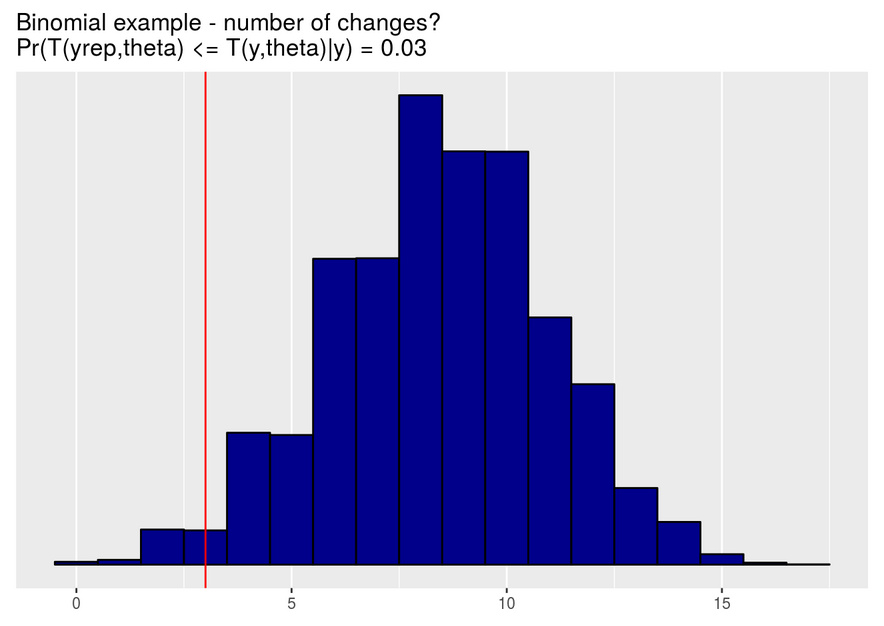
\includegraphics[width=80mm]{switches_hist.png}
\end{center}


\end{frame}

\end{document} 


